\section{Cancelling common factors before expansion}
\label{sec:gamma-cancel}
The connected identity removes the need to generate an IBP system for the supported trees, but a large target batch still requires many rational coefficients. The preceding implementation expands integer shifts of individual Gamma ratios and then cancels their common linear factors. We instead collect and cancel complete Gamma factors across the full integral before producing any finite products. We also calculate the dimension-dependent part of each subintegral power and the reference-master arguments once per batch. Appendix~\ref{app:gamma-cancel} derives these steps from the same bubble and triangle identities.

For each common dimension coefficient $B$, the method combines the signed multiplicities of $\Gamma(A+Bd/2)$. Their sum vanishes in the target-to-master ratio. The finite-product identity in Appendix~\ref{app:gamma-cancel} then produces only intervals with nonzero net multiplicity. This avoids forming factors that would cancel later. Integer arithmetic keeps the result exact. The method uses the same master and physical domain as the preceding connected reduction, while other integrals retain the existing exact and learned Kira workflow.

We compare 34 distinct tree structures through thirteen loops, with a small and a large symbolic-scale batch for each structure. The small batch contains seven targets. The large batch contains 128 targets with physical powers up to four, except at one loop, where its full allowed set has 96 targets. Four further requests check the unchanged analytic and native paths. Each method runs five times in a fresh process, with rotated order and the same output procedure. The timer includes loading, recognition, coefficient calculation, output, and exit. Independent comparisons occur after timing. The control uses the preceding coefficient routine in the same application, which isolates the combined effect of early mathematical cancellation and shared batch calculations.

All 72 requests complete in every repetition. The 4,558 connected target entries agree exactly with the preceding canonical rational coefficients, and 612 independent Gamma evaluations pass at 80-digit precision with relative tolerance $10^{-60}$. The Gamma checks use three selected targets from each connected request at the three dimensions defined in Appendix~\ref{app:loop-tree}. They test the implementation of the proved identity and do not constitute new native high-loop reductions.

\begin{table}[!htbp]\centering\small
\caption{Complete application times for the cancellation comparison. Each total sums request medians from five repetitions. The interval resamples complete requests. A ratio below one denotes less time.}
\label{tab:gamma-cancel}
\begin{tabularx}{\linewidth}{@{}Yrrrr@{}}\toprule
Collection & Requests & Previous (s) & New (s) & Ratio\\\midrule
Large batches & 34 & 14.305 & 6.731 & 0.471 \\
Seven-target batches & 34 & 4.838 & 4.964 & 1.026 \\
Unchanged-path checks & 4 & 4.412 & 4.404 & 0.998 \\
All requests & 72 & 23.556 & 16.100 & 0.683 \\
\bottomrule\end{tabularx}\end{table}

For the large connected batches, the new method uses 52.9\% less total time, with ratio 0.471 and request-resampling interval $[0.414,0.540]$. All 34 large requests have a shorter median time. The seven-target ratio is 1.026, with request-resampling interval $[0.986,1.071]$ and 17 slower requests. These short calls include loading and output, so a faster coefficient calculation need not produce a proportional saving in complete time. Across all 68 connected requests, time falls from 19.143 to 11.695 seconds. Including the four unchanged-path checks, total time falls from 23.556 to 16.100 seconds, or 31.7\% less time on this 72-request collection. The small-batch interval includes equal time, so the comparison does not resolve an improvement for short calls. These savings arise from exact simplification and shared calculation within a batch. The trained native choices remain unchanged, so this comparison does not assign the added gain to ML. It also preserves the preceding coverage limits for massive and multi-scale graphs.

\begin{figure}[!htbp]\centering
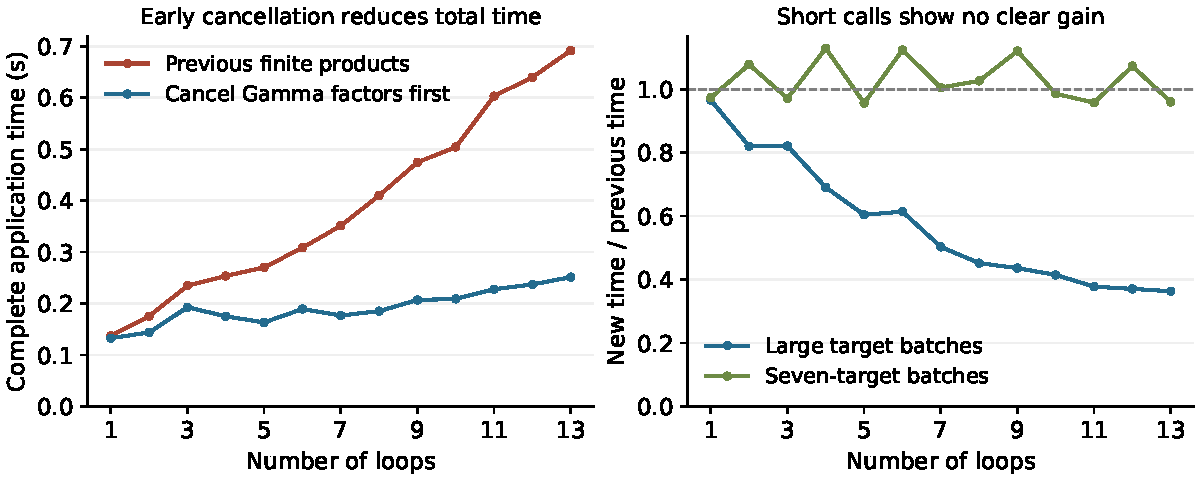
\includegraphics[width=\linewidth]{paper_figures/gamma_cancellation.pdf}
\caption{Early cancellation reduces complete time as the coefficient algebra grows. The left panel averages large-batch request medians at each loop order. The right panel divides summed new medians by summed control medians separately for each batch size. The one-loop large batch has 96 targets; the other large batches have 128. Each point compares matching structures and targets.}
\label{fig:gamma-cancel}
\end{figure}
\FloatBarrier
